%%%%%%%%%%%%%%%%%%%%%%%%%%%%%%%%%%%%%%%%%%%%%%%%%%%%%%%%%%%%%%%%%%%%%%%%%%%%%%%%

\documentclass[letterpaper, 10 pt, conference]{ieeeconf}


\IEEEoverridecommandlockouts                           
\overrideIEEEmargins    

\usepackage{times}
% numbers option provides compact numerical references in the text. 
\usepackage{graphics} % for pdf, bitmapped graphics files
\usepackage{mathtools}
\usepackage{graphicx}
\usepackage{tabularx}
\usepackage{caption}
% \usepackage{subcaption}
\usepackage{wrapfig}
\usepackage{romannum}
\usepackage{amsmath,amssymb}
% \usepackage{amsmath}
\usepackage{url}
\usepackage{bm}
\usepackage{bbm}
\usepackage[table,xcdraw]{xcolor}
\usepackage{hyperref}
\usepackage{subfigure}
\usepackage{cite}
\usepackage{amsthm}
\newtheorem{assumption}{Assumption}
\newtheorem{problem}{Problem}
\newtheorem{lemma}{Lemma}
\newtheorem{proposition}{Proposition}

\newcommand{\Tref}[1]{Table~\ref{#1}}
\newcommand{\Eref}[1]{Eq.~(\ref{#1})}
% \newcommand{\Eref}[1]{(\ref{#1})}
\newcommand{\Fref}[1]{Fig.~\ref{#1}}
\newcommand{\Sref}[1]{Section~\ref{#1}}

\usepackage{multirow}
\usepackage{booktabs}
\usepackage{pifont}
\usepackage{arydshln}
% \newcommand{\cmark}{\ding{51}}%
% \newcommand{\xmark}{\ding{55}}%
\usepackage{tabularx}
    % \newcolumntype{L}{>{\raggedright\arraybackslash}X}

\usepackage[ruled,vlined]{algorithm2e}
\usepackage[noend]{algpseudocode}
\makeatletter
\let\OldStatex\Statex
\renewcommand{\Statex}[1][3]{%
  \setlength\@tempdima{\algorithmicindent}%
  \OldStatex\hskip\dimexpr#1\@tempdima\relax}
\renewcommand{\ALG@beginalgorithmic}{\normalsize}

\renewcommand{\labelenumi}{\roman{enumi})}
\newcommand{\fu}{\frac{\partial \vf}{\partial \vu}}
\DeclareMathOperator{\Tr}{Tr}
\newcommand{\Pas}[2]{\mathcal{P}\left({#1}|{#2}\right)}
\newcommand{\Pol}[2]{\mathcal{U}\left({#1}|{#2}\right)}
\newcommand{\PolOpt}[2]{\mathcal{U}^{*}\left({#1}|{#2}\right)}
\newcommand{\PolPasT}[1]{\mathcal{P}\left({#1}\right)}
\newcommand{\PolT}[1]{\mathcal{U}\left({#1}\right)}
\newcommand{\traj}{\mathbf{X}}
\newcommand{\KL}[2]{\mathbb{D}_{\mathrm{KL}}\left({#1}\parallel {#2}\right)}
\newcommand{\costt}[1]{\mathcal{J}\left({#1}\right)}
\newcommand{\logb}[1]{\log\left({#1}\right)}
\newcommand{\expb}[1]{\exp\left({#1}\right)}
\newcommand{\val}[2]{\mathit{V}_{#2}\left({#1}\right)}
\newcommand{\zt}[2]{\Phi_{#2}\left({#1}\right)}
\newcommand{\nZ}[2]{\mathcal{G}_t[\Phi]\left({#1}\right)}
\newcommand{\ExP}[2]{\E_{{#1}}{\left[#2\right]}}
\newcommand{\vnu}{{\bf \nu}}
\newcommand{\pluseq}{\mathrel{+}=}
\newcommand{\cmark}{\ding{51}}%
\newcommand{\xmark}{\ding{55}}%

\DeclareCaptionFont{mysize}{\fontsize{8}{9.6}\selectfont}
\captionsetup{font=mysize}

%%%%%%%%%%%%%%%%%%%%%%%%%%%%%%%%%%%%%%%%%%%%%%%%%%%%%%%%%%%%%%%%%%%%%%%%%%%%%%%%
\title{\LARGE \bf Energy-Guided Priority under Battery Uncertainty \\ for Multi-Robot Coordination}

% \author{Anonymous Authors}
\author{Hoseong Jung, Sungil Son, Inkyu Jang, H. Jin Kim, Jungwon Park$^{*}$
% \thanks{This work was supported by Institute of Information \& communications Technology Planning \& Evaluation (IITP) grant funded by the Korean Government (MIST)}
\thanks{Hoseong Jung, Sungil Son, and H. Jin Kim are with Seoul National University, South Korea
        {\tt\footnotesize \{ghtjdaleka, aldridge99, hjinkim\}@snu.ac.kr}.}       
\thanks{Inkyu Jang is with the University of California, Berkeley, USA {\tt\footnotesize janginkyu.larr@gmail.com}.}
\thanks{Jungwon Park is with Seoul National University of Science and Technology, South Korea {\tt\footnotesize jungwonpark@seoultech.ac.kr}.}
\thanks{$^*$Corresponding author}}%

\begin{document}

\maketitle

%%%%%%%%%%%%%%%%%%%%%%%%%%%%%%%%%%%%%%%%%%%%%%%%%%%%%%%%%%%%%%%%%%%%%%%%%%%%%%%%

\begin{abstract}
As multi-agent systems transition from structured environments to unpredictable domains, communication constraints and energy autonomy become critical operational bottlenecks.
Furthermore, heterogeneous usage introduces battery uncertainty across identical hardware, complicating reliable planning.
To address these challenges, we explicitly calibrate this usage-induced uncertainty to enable a highly scalable, low-bandwidth coordination strategy.
We explore right-of-way coordination as a downstream task, where exchanging the energy sufficiency margin serves as a precedence cue during close encounters.
Specifically, future energy needs are estimated via a cell-specific proxy model, with prediction errors rigorously calibrated using adaptive conformal inference.
These calibrated margins dictate a unique yielding order, embedded into a responsibility-aware control barrier function (CBF) to enforce asymmetric collision avoidance.
While validations show this precedence cue maintains safety with slight energy efficiency gains during local encounters, the calibrated framework is ultimately more suited for comprehensive mission planning to achieve true long-term autonomy in the wild.

\end{abstract}

%%%%%%%%%%%%%%%%%%%%%%%%%%%%%%%%%%%%%%%%%%%%%%%%%%%%%%%%%%%%%%%%%%%%%%%%%%%%%%%%
\section{INTRODUCTION}\label{sec:intro}
\subsection{Motivation}
Deploying multi-agent systems in unstructured environments represents a critical frontier for modern autonomous systems beyond structured workspaces~\cite{yoshitake2019new, krnjaic2024scalable}.
Unlike controlled settings that benefit from reliable communication infrastructure, field deployments are fundamentally limited by intermittent networks and bounded energy reserves~\cite{mathew2015multirobot, calvo2025heterogeneous}.
When agents cross paths in these shared environments, their coupled motions require a decentralized right-of-way decision to determine which agent should proceed and which should yield~\cite{thomas2019right, celi2019deconfliction}.
In conventional approaches, resolving these spatial conflicts and preventing deadlocks requires bandwidth-intensive exchanges of complex planned trajectories or future task intents~\cite{wu2025decentralized, grover2023before}.
To drastically minimize this communication overhead, we propose energy-guided priority as a highly scalable coordination strategy. 
By exchanging only the energy sufficiency margin that predicts the energy remaining after task completion, agents can establish a unique, pairwise yielding order without relying on heavy trajectory sharing~\cite{notomista2018persistification, notomista2020persistification}.
This metric naturally scales to field constraints like sparse charging and complex missions, serving as a robust yielding cue for lifelong autonomy.

While this energy-guided priority is communication-efficient, its practical application must account for battery dynamics over long-term operations.
In practice, heterogeneous usage profiles naturally cause cell-specific battery degradation, introducing uncertainty even among identical hardware specifications. 
Rather than treating this uncertainty as a critical failure point, we seek to explicitly calibrate it to maintain a consistent and reliable precedence cue.

In this work, we estimate future energy requirements via a cell-specific proxy model and bound the residual prediction errors using adaptive conformal inference~\cite{gibbs2021adaptive}.
The resulting calibrated margins determine the discrete yielding order.
We then embed this precedence into a responsibility-aware control barrier function (CBF) formulation~\cite{cosner2023learning}.
Fig.~\ref{fig:main-figure} illustrates the overall idea: calibrated energy margins establish the yielding order, which is subsequently reflected in collision-avoidance responsibility.

\begin{figure*}[h!]
\centering
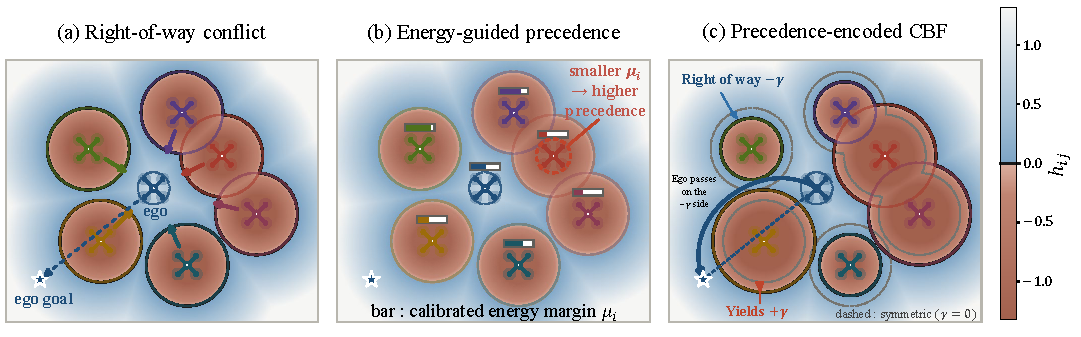
\includegraphics[width=\textwidth]{Figures/fig1_poc.pdf}
\caption{Energy-guided right-of-way coordination. (a) Multiple robots compete for right of way in a congested encounter. (b) Calibrated precedence cues $\mu_i$ determine a unique yielding order, where smaller $\mu_i$ indicates higher precedence and larger $\mu_i$ indicates greater flexibility to yield. (c) The order is encoded through a responsibility-aware CBF term ($\gamma$), assigning greater avoidance responsibility to the yielding robot while preserving pairwise safety.
\vspace{-10pt}
}
\label{fig:main-figure}
\end{figure*}

\subsection{Summary of Contributions}

We develop an uncertainty-calibrated energy-guided precedence rule for multi-robot right-of-way coordination and implement it using a responsibility-aware CBF formulation. 
Our main contributions are summarized as follows.

\textbf{Energy Sufficiency as a Precedence Criterion.} 
We use the energy expected to remain after task completion and travel to a charging station to determine pairwise right-of-way.
By exchanging only this scalar, agents establish a unique yielding order based on energy conditions, reducing communication overhead for conflict resolution.

\textbf{Uncertainty-Calibrated Energy Estimates.} 
We estimate the energy required to reach a charging station directly and after completing the assigned task using a battery-specific proxy model.
Adaptive conformal inference converts these predictions into bounds whose long-run violation rate is controlled at a prescribed level.
The resulting bounds define conservative precedence margins and an energy-sufficiency certificate with a conditional station-reachability guarantee.

\textbf{Safety-Preserving Precedence Integration.} 
We encode the precedence in a responsibility-aware CBF formulation by assigning unequal avoidance contributions within each interacting pair.
The paired local constraints preserve the underlying collision-avoidance condition regardless of which robot yields.
When multiple local right-of-way conflicts arise, all pairwise decisions follow a common energy-based ordering, thereby preventing cyclic precedence.


\subsection{Limitations and Future Works}
Our evaluations validate the efficacy of the energy-guided precedence cue within localized multi-agent encounters. 
However, confining this calibrated margin exclusively to a CBF formulation is inherently myopic for system-wide energy optimization. 
To achieve lifelong energy autonomy in disaster scenarios, future work will integrate this framework into higher-level mission planning architectures, such as global task allocation and long-horizon pathfinding.
%%%%%%%%%%%%%%%%%%%%%%%%%%%%%%%%%%%%%%%%%%%%%%%%%%%%%%%%%%%%%%%%%%%%%%%%%%%%%%%%

%%%%%%%%%%%%%%%%%%%%%%%%%%%%%%%%%%%%%%%%%%%%%%%%%%%%%%%%%%%%%%%%%%%%%%%%%%%%%%%%
% \section{Background and Related Works}\label{sec:rel_works}
% \subsection{Control Barrier Functions and Responsibility Allocation}\label{sec:2.A}
% Consider a control-affine system $\dot{x} = f(x) + g(x)u$, where $x \in \mathcal{X}\subseteq \mathbb{R}^n$, $u\in\mathcal{U}\subseteq\mathbb{R}^m$, $f$ and $g$ are locally Lipschitz, and $\mathcal{U}$ is a convex polytope.
Let $h:\mathcal{D}\rightarrow\mathbb{R}$ be continuously differentiable on an open domain $\mathcal{D}$ and define the safe set~as
\begin{equation}
    \mathcal{S} = \{\, x \in \mathcal{D} : h(x) \ge 0 \,\}.
    \label{eq:safe_set}
\end{equation}
The function $h$ is a control barrier function (CBF) if there exists an extended class-$\mathcal{K}$ function $\alpha$ such that
\begin{equation}
    \sup_{u\in\mathcal{U}}\big[ L_f h(x) + L_g h(x)u \big]\geq -\alpha\big(h(x)\big)
    \quad \forall x \in \mathcal{D},
    \label{eq:cbf_condition}
\end{equation}
where $L_f h = \nabla h^\top f$ and $L_g h = \nabla h^\top g$ are the Lie derivatives of $h$.
Under standard regularity conditions, any locally Lipschitz controller satisfying the corresponding CBF constraint renders $\mathcal{S}$ forward invariant~\cite{ames2019control}.

In multi-agent safety, responsibility quantifies how much each agent is expected to contribute to maintaining a shared constraint.
Existing CBF-based methods derive this allocation from social preferences, contextual interaction data, or collision risk~\cite{lyu2022responsibility, cosner2023learning, remy2025learning, lyu2023risk}.
For a pair with shared barrier $h_{ij}$, a responsibility-aware CBF requires agent $i$ to enforce
\begin{equation}
    L_{g_i} h_{ij} u_i + \frac{1}{2}(L_{f_{ij}}h_{ij} + \alpha_c (h_{ij})) - \gamma_{ij} \geq 0,
    \label{eq:responsibility_cbf}
\end{equation}
where $L_{f_{ij}} h_{ij}$ collects the drift contributions of both agents.
A larger $\gamma_{ij}$ tightens the constraint and assigns agent $i$ a greater safety-preserving contribution.
When $\gamma_{ji}=-\gamma_{ij}$, the paired constraints recover the standard CBF condition when summed.
In this work, we use this allocation to encode energy-guided precedence: the yielding robot receives greater collision-avoidance responsibility.
% \subsection{Energy Sufficiency for Persistent Robot Operation}\label{sec:2.B}
% Energy-aware autonomy is essential for sustaining long-duration robot operation under finite battery capacity.
Persistification methods formalize this objective by preserving the set of states from which recharging remains feasible before energy depletion~\cite{notomista2018persistification, notomista2020persistification}, including extensions to multi-robot systems with shared charging resources~\cite{fouad2022energy}.
Related approaches sustain long-duration autonomy through recharge rendezvous and shared-station scheduling~\cite{mathew2015multirobot, kumar2025persistent}.
While these works use energy information primarily to maintain continued operation, we use the energy-sufficiency margin as a right-of-way criterion.
A larger margin indicates greater flexibility to accommodate an avoidance detour.
We therefore assign the robot with the larger margin to yield.
% \subsection{Adaptive Conformal Inference}\label{sec:2.C}
% Conformal prediction constructs prediction sets by calibrating a scalar measure of discrepancy between predictions and observations~\cite{shafer2008tutorial}.
This quantity is referred to as a nonconformity score.
Let $\widehat{y}_t$ denote a point prediction of an outcome $y_t$, and define
\begin{equation}
    s_t=S(y_t, \widehat{y}_t),
\end{equation}
where $S$ is an application-dependent score function.
Let $q_t(\beta)$ denote the empirical $(1-\beta)$-quantile of the previously observed scores with the standard finite-sample correction.
The corresponding prediction set is
\begin{equation}
    \mathcal{C}_t(\beta)=\{
    y:S(y, \widehat{y}_t)\leq q_t(\beta) \}.
    \label{eq:conformal_set}
\end{equation}
Under exchangeability of the calibration and test scores, $\mathcal{C}_t(\beta)$ provides marginal coverage of at least $1-\beta$.

In sequential robotic operation, the score distribution may vary over time and exhibit temporal dependence.
Adaptive conformal inference adjusts the effective miscoverage level using observed violations~\cite{gibbs2021adaptive}.
Let $e_t=\mathbbm{1}\{y_t\notin\mathcal{C}_t(\beta_t)\}$ denote a prediction-set violation.
For a target violation level $\delta$, the adaptive update is
\begin{equation}
    \beta_{t+1} = \beta_t + \eta(\delta-e_t),
    \label{eq:adaptive_conformal_update}
\end{equation}
where $\eta>0$ is the adaptation rate.
A violation decreases $\delta_t$ and enlarges subsequent prediction sets, whereas repeated coverage permits tighter sets.
This feedback controls the long-run empirical violation frequency rather than guaranteeing coverage for every individual prediction.

Adaptive conformal methods have been applied to motion planning and safety-critical control to calibrate trajectory-prediction and safety-assessment errors online~\cite{zhou2024safety, huriot2026safe}.
In~this work, we use the upper-tail prediction error of a future energy requirement as the score.
Its calibrated quantile yields a one-sided upper bound used to define the energy-sufficiency certificate and precedence margin.

\section{Problem Formulation}\label{sec:problem_formulation}
This section presents the multi-robot right-of-way problem under uncertain battery conditions. 
We first define the robot motion, battery state, and future energy requirements for task completion and station reachability (Sec.~\ref{sec:3.A}). 
We then formulate the energy-guided precedence and safety objectives (Sec.~\ref{sec:3.B}).
\subsection{Motion and Energy Dynamics}\label{sec:3.A}
Consider a team of $N$ robots, indexed by $\mathcal{A}=\{1, \ldots, N\}$.
Robot $i$ follows the control-affine dynamics
\begin{equation}
    \dot{x}_i = f_i(x_i) + g_i (x_i)u_i, \quad u_i \in\mathcal{U}_i
    \label{eq:motion_dynamics}
\end{equation}
where $x_i \in \mathcal{X}_i$ is the robot state, $\mathcal{U}_i$ is a convex input set, and $f_i$ and $g_i$ are locally Lipschitz.
Let $p_i=\Pi_i x_i$ denote the robot position.
Each robot is assigned a task goal $p_i^g$ and may recharge at one of the stations $\mathcal{C}=\{c_1, \ldots, c_K\}$.

We represent the battery state of robot $i$ by its filtered load voltage $V_i$, which serves as a measurable proxy for remaining energy.
Let $V_{\min}$ denote the minimum operational voltage, and define the augmented state
\begin{equation}
    z_i := [x_i^\top, V_i]^\top.
    \label{eq:augmented_state}
\end{equation}
For each station $c_k$, let $c_{i,k}^{\mathrm{sta}}(z_i)$ denote the future voltage cost of traveling directly to $c_k$, and let $c_{i,k}^{\mathrm{task}}(z_i)$ denote the cost of completing the assigned task and subsequently reaching $c_k$.
These trajectory-level costs depend on the current motion and battery states and are unknown at the time of coordination.
\subsection{Problem Statement}\label{sec:3.B}
For multi-robot right-of-way coordination, we aim to 1) construct uncertainty-calibrated upper bounds for future energy requirements; 
2) use these bounds to determine a unique energy-guided yielding order; and
3) encode the resulting order via responsibility-aware CBF constraints while preserving pairwise collision avoidance.
The problem is formulated as follows.

\begin{problem}[Energy-Guided Right-of-Way Coordination]
\label{prob:main}
Given the robot dynamics in Eq.~\eqref{eq:motion_dynamics}, the measured augmented states $\{z_i\}_{i\in\mathcal{A}}$, and a target violation level $\delta\in(0,1)$, construct calibrated future-cost bounds and control inputs satisfying the following requirements.

\begin{enumerate}
    \item \textbf{Uncertainty-calibrated energy bounds:} for each calibrated sequence of future energy requirements $\{c_\ell\}$, construct upper estimates $\{\bar{c}_\ell\}$ such that
    \begin{equation}
        \limsup_{L\rightarrow\infty}\frac{1}{L}\sum_{\ell=1}^L\mathbbm{1}\{c_\ell>\bar{c}_\ell\}\leq \delta.
        \label{eq:target_violation_rate}
    \end{equation}

    \item \textbf{Energy-guided precedence:} Using the uncertainty-calibrated future energy estimates, construct energy-based precedence scores $\{\mu_i\}_{i\in\mathcal{A}}$ that reflect each robot's flexibility to accommodate the additional cost of yielding. For every interacting pair $(i, j)$, the robot with the larger score is assigned to yield, with ties resolved by a fixed rule. When multiple conflicts arise, all pairwise decisions follow the common ordering induced by $\{\mu_i\}_{i\in\mathcal{A}}$.
    
    \item \textbf{Safety-preserving precedence integration:} encode the selected yielding order through complementary responsibility allocations while ensuring
    \begin{equation}
        h_{ij}(x_i(0), x_j(0)) \geq 0 \Longrightarrow h_{ij}(x_i(t),x_j(t))\geq 0,
        \label{eq:pairwise_safety_objective}
    \end{equation}
    for all $t\geq 0$ and every interacting pair $(i, j)$.
    % When multiple conflicts arise, all pairwise decisions follow the common ordering induced by $\{\mu_i\}_{i\in\mathcal{A}}$.
    
\end{enumerate}

\end{problem}
\section{Method}
This section solves Problem~\ref{prob:main} in two stages:
uncertainty-calibrated energy-based precedence cue (Sec.~\ref{sec:4.A}), and safety-preserving precedence integration (Sec.~\ref{sec:4.C}).
The overall procedure of our approach is summarized in Fig.~\ref{fig:method}.

\begin{figure*}[t!]
\centering
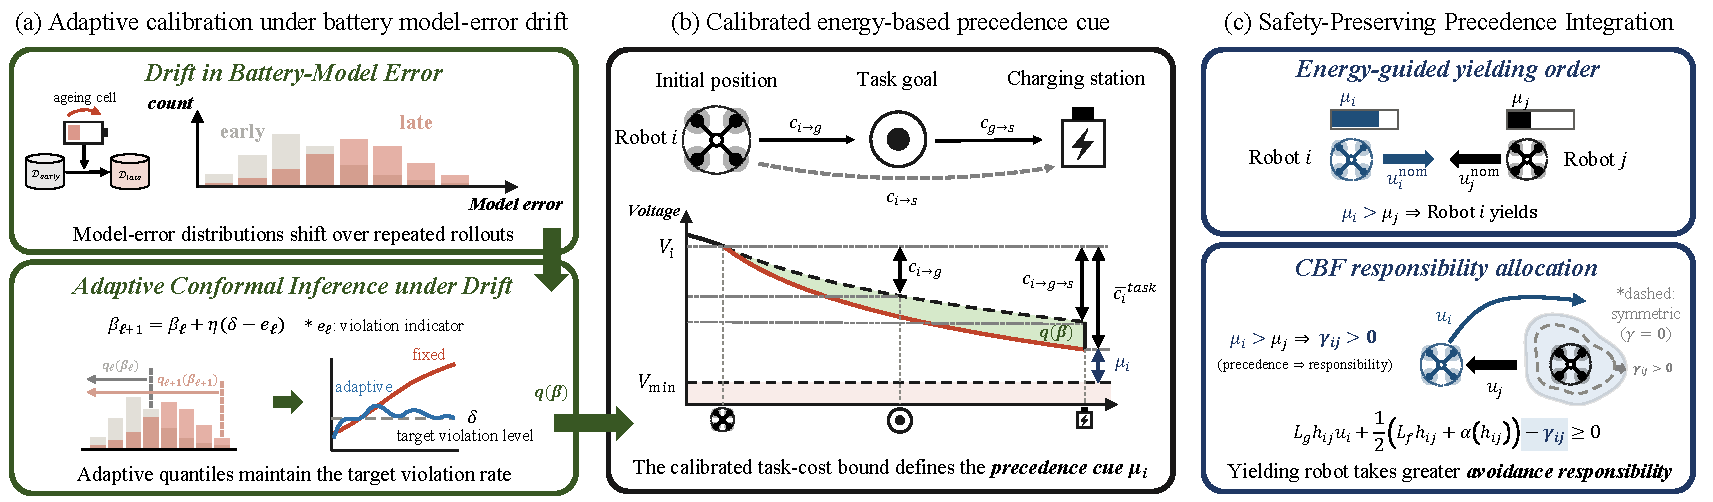
\includegraphics[width=\textwidth]{Figures/fig2.pdf}
\caption{Overview of the proposed energy-guided precedence framework. (a) Adaptive conformal inference calibrates battery-model error under distribution shift, producing an adaptive quantile $q_\ell(\beta_\ell)$ at the target violation level. (b) The calibrated task-cost bound defines the energy-based precedence cue $\mu_i$. (c) The resulting yielding order is encoded through CBF responsibility allocations, so the yielding robot assumes greater avoidance responsibility while pairwise safety is preserved.
\vspace{-10pt}
}
\label{fig:method}
\end{figure*}
\subsection{Uncertainty-Calibrated Precedence Cue}\label{sec:4.A}
To establish a low-bandwidth yielding order, we define the energy sufficiency margin $\mu_i$ as the calibrated estimate of remaining energy after task completion. 
Let $c_l$ denote the true future energy cost and $\hat{c}_l$ be the prediction from a cell-specific proxy model. 
To handle usage-induced battery uncertainty, we calibrate the residual error $s_l = c_l - \hat{c}_l$ using adaptive conformal inference~\cite{gibbs2021adaptive}. 
Specifically, the adaptive quantile $q_l(\beta_l)$ is computed as the empirical $(1-\beta_l)$-quantile of the previously observed calibration scores.
This feedback mechanism dynamically adjusts the effective miscoverage level: a bound violation decreases $\beta$ to enlarge subsequent prediction bounds, whereas repeated coverage permits tighter margins.
Consequently, the online update maintains a target violation rate $\delta$ even under distribution shifts caused by cell degradation:
\begin{equation}
    \beta_{l+1} = \beta_l + \eta(\delta - \mathbbm{1}\{c_l > \hat{c}_l + q_l(\beta_l)\}).
\end{equation}
The resulting calibrated task-cost bound $\overline{c}_i^{task}$ defines the precedence margin:
\begin{equation}
    \mu_i = V_i - V_{min} - \overline{c}_i^{task},
\end{equation}
where $V_i$ is the current voltage and $V_{min}$ is the minimum operational threshold. 
For any interacting pair $(i, j)$, the agent with the larger margin has greater flexibility and is assigned to yield (i.e., $\mu_i > \mu_j \implies i \text{ yields to } j$). 
% Let $\tau\in\mathcal{T}:=\{\mathrm{sta},\mathrm{task}\}$ denote the trajectory type.
% For robot $i$ and station $c_k$, let $\xi_{i,k}^{\tau}$ denote the planned trajectory reaching $c_k$ directly when $\tau=\mathrm{sta}$, or after task completion when $\tau=\mathrm{task}$.
% The battery-specific proxy model
% \begin{equation}
%     \dot{\widehat V}_i=
%     \widehat f_{V,i}(z_i;\theta_i)
%     +\widehat g_{V,i}(z_i;\theta_i)^\top u_i
%     \label{eq:proxy_voltage_model}
% \end{equation}
% predicts the voltage evolution along $\xi_{i,k}^{\tau}$, where $\theta_i$ contains robot-specific model parameters.
% The resulting point estimate of the future voltage cost is
% \begin{equation}
%     \widehat c_{i,k}^{\tau}
%     :=V_i-\widehat V_{i,k}^{\tau}(H_{i,k}^{\tau}),
%     \label{eq:predicted_voltage_cost}
% \end{equation}
% where $H_{i,k}^{\tau}$ is the trajectory horizon.

% We calibrate the residual proxy-model error separately for each robot and trajectory type.
% For clarity, these indices are omitted below.
% Let $\ell$ index completed trajectories, and define the upper-tail score
% \begin{equation}
%     s_\ell:=c_\ell-\widehat c_\ell.
%     \label{eq:energy_nonconformity_score}
% \end{equation}
% Let $q_\ell(\beta)$ denote the finite-sample-corrected empirical $(1-\beta)$-quantile of the previously observed scores.
% For a prediction issued at calibration round $\ell$, the calibrated one-sided upper prediction bound is
% \begin{equation}
%     \overline c_{i,k}^{\tau}
%     :=\widehat c_{i,k}^{\tau}
%     +q_\ell(\beta_\ell).
%     \label{eq:calibrated_energy_bound}
% \end{equation}
% After the realized cost becomes available, define
% \begin{equation}
%     e_\ell:=\mathbbm{1}\{c_\ell>\overline c_\ell\},
%     \;
%     \beta_{\ell+1}:=\beta_\ell+\eta(\delta-e_\ell),
%     \label{eq:energy_aci_update}
% \end{equation}
% where $\delta$ is the target violation level and $\eta>0$ is the adaptation rate.
% A bound violation decreases $\beta_\ell$ and increases the subsequent quantile, whereas repeated coverage permits tighter bounds.
% Summing the update gives
% \begin{equation}
%     \frac{1}{L}\sum_{\ell=1}^{L}e_\ell-\delta
%     =\frac{\beta_1-\beta_{L+1}}{\eta L}.
%     \label{eq:aci_violation_identity}
% \end{equation}
% Thus, if the adaptive levels remain bounded, the empirical violation frequency converges to the prescribed level $\delta$.
% Consequently, the calibrated bounds in Eq.~\eqref{eq:calibrated_energy_bound} satisfy the uncertainty-calibrated energy-bound requirement of Problem~\ref{prob:main}.
% These bounds are used next to construct the energy-sufficiency certificate and precedence margin.
% \subsection{Energy Sufficiency and Precedence}\label{sec:4.B}
% Using the calibrated bounds in Eq.~\eqref{eq:calibrated_energy_bound}, define the minimum calibrated cost bound for each trajectory type as
\begin{equation}
    \overline c_i^\tau:=\min_{k\in\{1,\ldots,K\}}\overline c_{i,k}^\tau,
    \qquad
    k_i^\tau\in\arg\min_k \overline c_{i,k}^\tau,
    \label{eq:minimum_calibrated_cost}
\end{equation}
where station ties are resolved by a fixed rule.
The station-reachability certificate and energy margin are then defined~as
\begin{equation}
    h_{e,i}=V_i-V_{\min}-\overline c_i^{\mathrm{sta}},
    \qquad
    \mu_i=V_i-V_{\min}-\overline c_i^{\mathrm{task}}.
    \label{eq:calibrated_energy_quantities}
\end{equation}
If $h_{e,i}\geq0$ and the station-cost bound is not violated, then
\begin{equation}
    V_i - V_{\min}-c_{i, k_i^\mathrm{sta}}^{\mathrm{sta}}
    \geq V_i - V_{\min} -\overline{c}_{i, k_i^{\mathrm{sta}}}^{\mathrm{sta}} = h_{e, i} \geq 0.
    \label{eq:conditional_station_reachability}
\end{equation}
Thus, $h_{e,i}\geq0$ provides a conditional certificate that robot $i$ can reach the selected station without falling below $V_{\min}$.
At runtime, $h_{e,i}$ is evaluated as an online station-reachability certificate, but is not imposed as a control constraint.

For right-of-way coordination, a larger $\mu_i$ indicates greater flexibility to accommodate the additional cost of yielding.
For an interacting pair $(i,j)$, define
\begin{equation}
    i\rightarrow j
    \quad\Longleftrightarrow\quad
    \mu_i>\mu_j
    \;\;\text{or}\;\;
    \bigl(\mu_i=\mu_j \text{ and } i>j\bigr),
    \label{eq:energy_precedence}
\end{equation}
where $i\rightarrow j$ means that robot $i$ yields to robot $j$.
Because the margins and robot indices define a strict total order, each interacting pair receives exactly one yielding direction.
Any subset of pairwise relations induced by this order is therefore acyclic.
The robot index is used only when the calibrated margins are equal; all non-tied decisions are determined by the energy-sufficiency margins.
The ordering in Eq.~\eqref{eq:energy_precedence} satisfies the energy-guided precedence requirement of Problem~\ref{prob:main}.

\subsection{Safety-Preserving Precedence Integration}\label{sec:4.C}
To enforce this discrete precedence order at the continuous control level, we embed it into a responsibility-aware control barrier function (CBF)~\cite{cosner2023learning}. 
We define a directional indicator $\psi_{ij} \in \{-1, 1\}$ based on the yielding order and allocate an asymmetric avoidance responsibility $\gamma_{ij} = \rho \psi_{ij}$.
The yielding agent takes on a tighter constraint within the local quadratic program (QP):
\begin{equation}
    L_{g_i}h_{ij}u_i + \frac{1}{2}(L_{f_{ij}}h_{ij} + \alpha(h_{ij})) - \gamma_{ij} \ge 0.
\end{equation} 
By exchanging only the scalar $\mu_i$, agents dynamically reallocate avoidance efforts without sharing future trajectories, strictly preserving pairwise collision avoidance. 

% The energy quantities in Sec.~\ref{sec:4.B} determine the discrete precedence, while the continuous control layer enforces the associated pairwise collision-avoidance constraints.
% For an interacting pair $(i,j)$, define the collision-avoidance barrier
% \begin{equation}
%     h_{ij}(x_i,x_j):=\|p_i-p_j\|^2-d_{\min}^2,
%     \label{eq:collision_barrier}
% \end{equation}
% where $d_{\min}>0$ is the required separation distance.
% Assuming relative degree one, the shared CBF condition is
% \begin{equation}
%     L_{f_{ij}}h_{ij}
%     +
%     L_{g_i}h_{ij}u_i
%     +
%     L_{g_j}h_{ij}u_j
%     +
%     \alpha_c(h_{ij})
%     \geq0.
%     \label{eq:shared_collision_cbf}
% \end{equation}
% We encode the precedence in Eq.~\eqref{eq:energy_precedence} through the directional variable
% \begin{equation}
%     \psi_{ij}
%     :=
%     \begin{cases}
%         1, & i\rightarrow j,\\
%         -1, & j\rightarrow i,
%     \end{cases}
%     \qquad
%     \psi_{ji}=-\psi_{ij}.
%     \label{eq:precedence_direction}
% \end{equation}
% Let $\rho_{ij}=\rho_{ji}>0$ denote the responsibility magnitude and set
% \begin{equation}
%     \gamma_{ij}:=\rho_{ij}\psi_{ij},
%     \qquad
%     \gamma_{ji}:=-\gamma_{ij}.
%     \label{eq:complementary_responsibility_terms}
% \end{equation}
% Because the local constraint contains $-\gamma_{ij}$, the yielding robot receives the tighter constraint and hence greater collision-avoidance responsibility.

% Let $\mathcal{N}_i^{\mathrm{act}}$ denote the robots currently interacting with robot $i$.
% Robot $i$ computes its control input from
% \begin{equation}
% \begin{aligned}
%     u_i^\star:=
%     \arg&\min_{u_i\in\mathcal U_i}\quad
%     \frac{1}{2}
%     \|u_i-u_i^{\mathrm{nom}}\|_{W_i}^{2}\\
%     \mathrm{s.t.}&\quad
%     L_{g_i}h_{ij}u_i
%     +
%     \frac{1}{2}
%     \left(
%         L_{f_{ij}}h_{ij}
%         +
%         \alpha_c(h_{ij})
%     \right)
%     -
%     \gamma_{ij}
%     \geq0,\\
%     &\hspace{52.5mm}
%     \forall j\in\mathcal N_i^{\mathrm{act}},
% \end{aligned}
% \label{eq:local_precedence_qp}
% \end{equation}
% where $u_i^{\mathrm{nom}}$ is the task-level reference input and $W_i\succ0$.
% For each pair $(i,j)$, summing the two local constraints and using $\gamma_{ij}+\gamma_{ji}=0$ recovers the standard pairwise CBF condition.
% Thus, the allocation changes which robot contributes more to collision avoidance without changing the underlying safety requirement.
% Each robot simultaneously enforces all active pairwise constraints in Eq.~\eqref{eq:local_precedence_qp}.
% Under standard CBF regularity and QP-feasibility conditions, the collision-free sets are forward invariant.
% The resulting controller therefore satisfies the safety-preserving precedence-integration requirement of Problem~\ref{prob:main}.
\section{Experiments}
This section validates the proposed framework in two stages: real-world battery calibration (Sec.~\ref{sec:5.A}), and hardware validation of energy-guided precedence (Sec.~\ref{sec:5.B}).
\subsection{Real-World Battery Calibration}\label{sec:5.A}
\textbf{Setup and Dataset.}
To capture realistic discharge statistics under dynamic flight profiles, we collected an extensive dataset using single-cell LiPo batteries from a Crazyflie 2.1 fleet.
Rather than relying on static bench tests, we compiled approximately 3 hours of active flight data across 200 distinct sorties, incorporating both standard demonstrations~\cite{ullah2026nanobench} and multi-sortie waypoint navigation tasks.
Crucially, the data was sourced from 14 individual battery cells, explicitly capturing the heterogeneous voltage drop characteristics encountered in physical deployments.
We fit a physically parameterized load-voltage proxy model to this dataset, evaluating the calibration performance using a strict held-out testing approach for each independent cell.

\textbf{Results.}
We evaluate whether adaptive conformal inference reliably maintains the one-sided energy bounds below the target violation level ($\delta=0.10$). 
As illustrated in Fig.~\ref{fig:fig3} (left), the adaptive framework successfully drives the empirical violation frequency below the target threshold over sequential calibration rounds.
Furthermore, when evaluated across all 14 individual battery cells under distribution shift, our adaptive method robustly bounds the error (Fig.~\ref{fig:fig3} (right)). 
In contrast, a standard fixed-quantile baseline fails to adapt to cell-specific degradation, resulting in uncalibrated bound violations with a mean of $0.116$ and a standard deviation of $0.114$. 
These comparative results confirm that our calibration layer effectively absorbs usage-induced discrepancies, producing a statistically sound energy-sufficiency margin to serve as a trustworthy precedence cue.

\begin{figure}[t!]
\centering
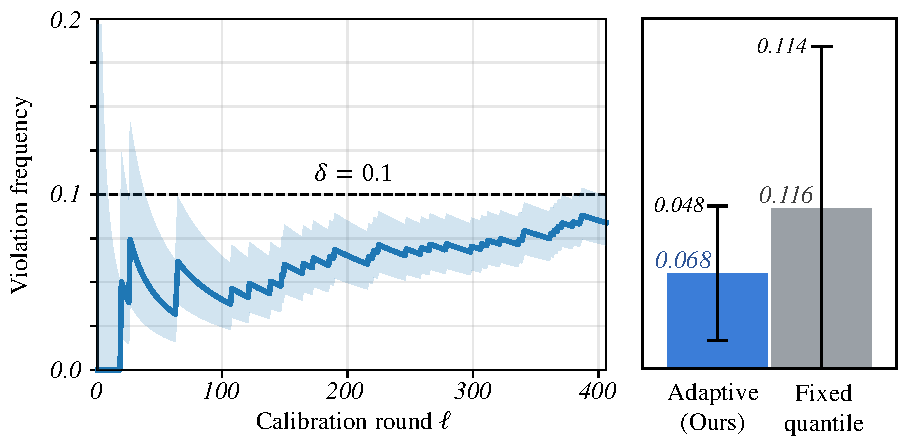
\includegraphics[width=\columnwidth]{Figures/fig3.pdf}
\caption{Battery calibration performance. \textbf{(Left)} The running violation frequency converges below the target $\delta=0.1$. \textbf{(Right)} Our adaptive method successfully bounds errors across 14 cells (mean $0.068$, std $0.048$), outperforming the fixed-quantile baseline.
}
\vspace{-10pt}
\label{fig:fig3}
\end{figure}
\subsection{Hardware Validation of Energy-Guided Precedence}\label{sec:5.B}
\textbf{Setup.} We deployed eight Crazyflie 2.1 quadrotors under an OptiTrack motion capture system to execute a dense position-exchange task, utilizing Crazyswarm to broadcast nominal trajectories~\cite{preiss2017crazyswarm}.
Given the close proximity of the congested intersection, agents reliably exchanged their standard local states (e.g., pose and velocity) alongside their individual calibrated energy margins. 
While the local state information was used to enforce a responsibility-aware CBF with a 0.4~m safety margin, the single scalar energy margin uniquely determined the pairwise yielding precedence. 
This critical separation allows agents to safely coordinate without relying on bandwidth-intensive trajectory sharing.

\textbf{Results and Implications.} Throughout the demonstration, this decentralized approach successfully resolved all spatial conflicts, resulting in zero collisions. 
As illustrated in Fig.~\ref{fig:fig4}, the precedence cue induced a strictly asymmetric yielding behavior: agents with lower energy margins (depicted in red) retained their right-of-way for direct traversal, whereas agents with higher margins (depicted in yellow) actively absorbed the collision-avoidance responsibility to yield safely. 
Ultimately, this experiment confirms that coupling safety-critical state feedback with a low-overhead, energy-guided priority signal provides a scalable, robust foundation for long-term multi-agent operations in the field.
%%%%%%%%%%%%%%%%%%%%%%%%%%%%%%%%%%%%%%%%%%%%%%%%%%%%%%%%%%%%%%%%%%%%%%%%%%%%%%%%
\section{CONCLUSION}
This work introduced an uncertainty-calibrated, energy-guided precedence rule for multi-agent right-of-way coordination.
To minimize communication overhead, we absorbed battery degradation via adaptive conformal inference and embedded this reliable cue into a control barrier function.
While hardware validations demonstrated its efficacy for decentralized collision avoidance, confining this metric exclusively to the reactive control layer remains myopic for system-wide optimization.
To achieve true energy autonomy, future work will integrate this framework into lifelong multi-agent reinforcement learning architectures for global task allocation in disaster scenarios.
\addtolength{\textheight}{0cm}   % This command serves to balance the column lengths
                                  % on the last page of the document manually. It shortens
                                  % the textheight of the last page by a suitable amount.
                                  % This command does not take effect until the next page
                                  % so it should come on the page before the last. Make
                                  % sure that you do not shorten the textheight too much.


\bibliographystyle{IEEEtran}
\bibliographystyle{plainnat}

\bibliography{mybib.bib}

\begin{figure}[t!]
\centering
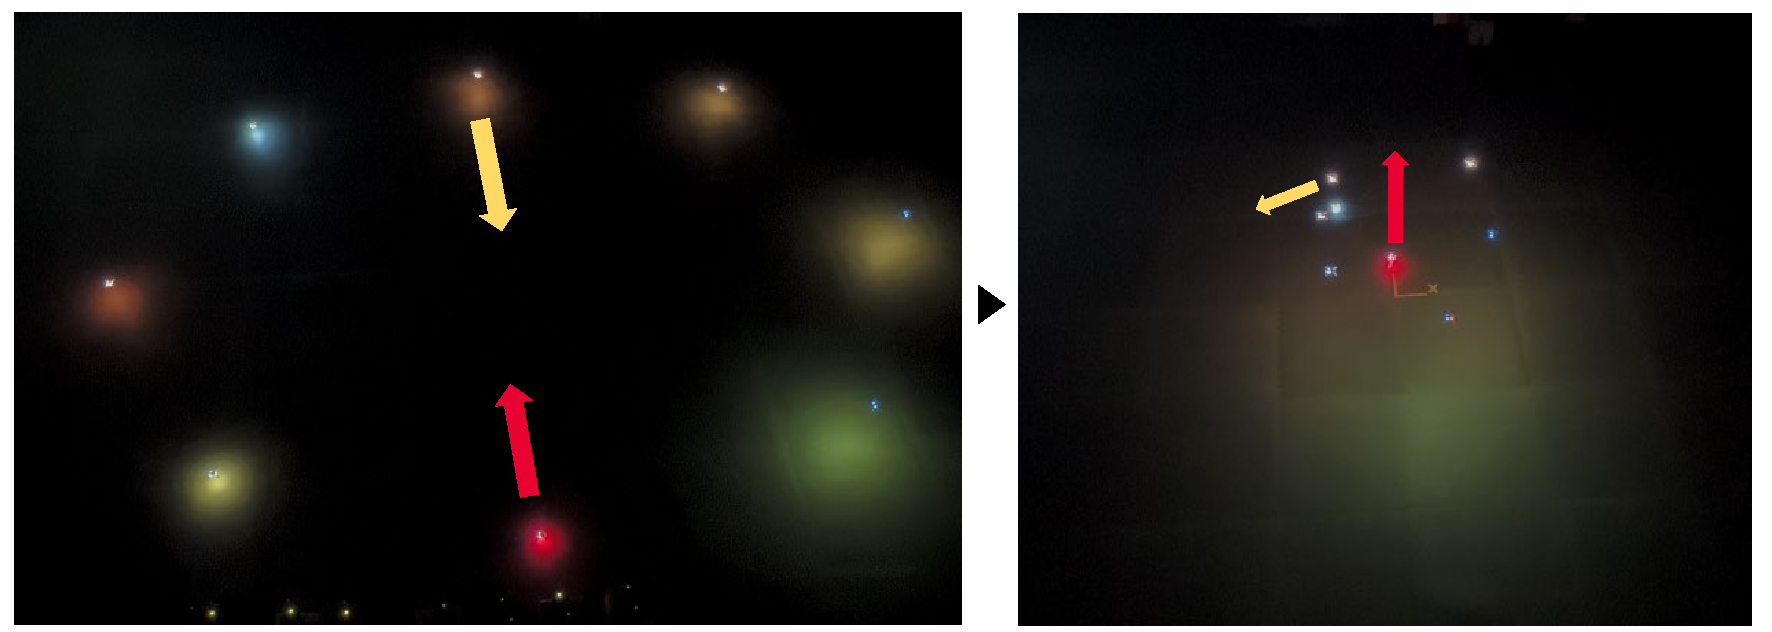
\includegraphics[width=\columnwidth]{Figures/fig4.pdf}
\caption{Hardware validation in an 8-agent congested intersection. \textbf{(Left)} Agents move to opposite positions, creating spatial conflicts. The red agent possesses a higher energy-guided priority than the yellow agent. \textbf{(Right)} Enforcing the calibrated precedence cue, the yellow agent actively yields, allowing the red agent to safely maintain its direct path.
}
\vspace{-10pt}
\label{fig:fig4}
\end{figure}

\end{document}